We implemented all the simple steering behaviours that were provided.
These are \textbf{seek}, \textbf{flee}, \textbf{arrive} and \textbf{wander}.
Last but not least we implemented two advanced steering behaviour: \textbf{obstacle avoidance} and \textbf{explore}.
Firstly, we will discuss every behaviour we implemented a little.
\subsection[Describing the steering behaviours]{Behaviours}\label{subsec:behaviours}
In this section I will talk about every behaviour slightly.
We will discuss our way of implementing each behaviour and how it works.
\subsubsection{Seek}
This was the first behaviour we implemented, simply because we thought this was the easiest behaviour to implement.
We couldn't have been more right.
The seek algorithm simply moves towards a goal at max speed, and will still be moving at max speed when arriving at the target.
Since it doesn't slow down, it just passes the goal, and then turns around to, again, reach towards this goal at max speed.
This results in moving bach and forth, through the goal.
\paragraph{Implementation}
Thus, the algorithm needs a goal (\textit{BaseGameEntity}), and a user, which we called movingEntity (\textit{MovingEntity}).
Having this goal, we could determine which direction the movingEntity should go to, in order to reach this goal.
Now, we can return a force (\textit{Vector2D}), equal to the max possible force for the current movingEntity.
To finish his behaviour, only the velocity our movingEntity currently has, has to be substracted from this force.
This way our entity won't make a sharp, but a smooth turn.
\subsubsection{Flee}
The flee behaviour is not much more than the seeking behaviour, but reversed.
With this I mean that in stead of moving towards a target at max speed, the entity moves away from a target at max speed.
One addition is that when there is an obstacle in between the target and our entity, the algorithm should just do nothing.
Unfortunately, the last part is not implemented yet.
\paragraph{Implementation}
First, we check if in between the entity and the goal is an obstacle present, if there is: do nothing!
If there isn't, go on with your calculation.
The calculation of the fleeing behaviour is almost exactly the same as the calculation of the seek behaviour.
Only, when you have found the direction you want to go in, you turn it around.
This is simply done by creating a new desired velocity, called newDesiredVelocity (\textit{Vector2D}), and inverting the X and the Y of the already found velocity.
\subsubsection{Arrive}
This is also a behaviour that is much like seek.
The difference is that, where seek continues to move with max speed at the target, the arrive behaviour will slow down till it reaches its target.
\paragraph{Implementation}
Actually, the implementation of the arrive behaviour is a lot different from seek.
Arrive also has to take the deceleration speed into account, and the distance between the moving entity and the target.
We have put a boundry on calculate this on a distance of 0.05, because everything after that will be unseeable movements and really specific calculations.
This is not needed.
The closer the entity is to the target, the slower it will be.
We achieve this by dividing the speed by the distance and multiplying that with the distance to our target, getting a desiredVelocity (\textit{Vector2D}).
Lastly, we have to substract the current velocity from the currentVelocity again.
\subsubsection{Wander}
Then, finally, we come across a more interesting behaviour, making it seem like the entity is wandering over the screen.
This wandering should happen as random as it could, and will be used when the entities have nothing much to do.
This way to do this is to get a \textbf{circle} at a certain distance in front of our entity, in the direction of our entity as well.
On this circle, choose a \textbf{point} to move towards, and make this point move along the circle in a random direction. (up and down)
\begin{figure}[h!]
    \begin{center}
        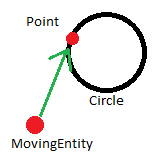
\includegraphics[width=10em]{WanderBehaviour.png}
    \end{center}
    \caption{Wander behaviour explanation example}
    \label{fig:WanderBehaviourExplanation}
\end{figure}
\paragraph{Implementation}
Looking at the image, it looks like a pain to implement, but it actually is quite easy!
To do it we actually need some extra variables, namely:
\begin{itemize}
    \item Circle distance
    \\\textit{The distance between the MovingEntity and the middle of the circle.}
    \item Circle radius
    \\\textit{The radius of the circle.}
    \item Turning angle
    \\\textit{The angle the point has to 'turn' when this value is calculated.}
    \item Previous angle
    \\\textit{To remember the previous of the dot (so we can move it from that point), we just remember the last angle inside a variable!}
\end{itemize}
First, you calculate the direction the entity currently goes to.
Somewhere inbetween you can change the angle to a new angle.
Since this should happen randomly, add or substract (chosen randomly) the turning angle from/to the previous angle.
Determine the middle of the circle and calculate the angle of where the piont should be.
Now just return the vector towards that point and you're done.
\subsubsection{Obstacle avoidance}\label{sec:ObstacleAvoidance}
All in all we spent the most time finding a solution to obstacle avoidance.
We will only explain how this behaviour works, and in a later part of this document we will talk about our problem.
A rectangle gets drawn in front of the movingEntity in the direction the entity goes to.
Within this rectangle, collisions with obstacles get checked.
If there is a collision with an obstacle, create a force in the opposite direction.
\begin{figure}[h!]
    \begin{center}
        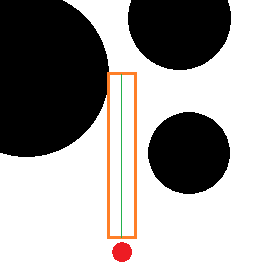
\includegraphics[width=10em]{ObstacleAvoidance.png}
    \end{center}
    \caption{Obstacle avoidance example}
    \label{fig:ObstacleAvoidanceExplanation}
\end{figure}
\paragraph{Implementation}
Compared to the explanation, the implementation is fairly complex.
This is because, when you have a lot of obstacles, it is really ineffici\"ent to check your collision with all the obstacles.
So, we filter the obstacles on being within the range of movingEntities current velocity in a list, \textit{obstaclesWithinRange}.
The rectangle drawn in front of our entity, only is as big as your own velocity, making it impossible to even reach obstacles that are further away than your velocity.
To see where each obstacle is compared to our entity, we translate these obstacles to our 'local space'.
This means nothing more than 'position compared to our entity its position'.
Do this by translating all obstacles in \textit{obstaclesWithingRange} with position of our current entity.
After you have translated these obstacles, rotate them according to the direction of our current moving entity.
If you have done this, all obstacles with a negative X value will be 'behind you'. (since, for the axial system, you rotated them relative to the right of our current entity)
For each obstacle in front of you and within your range, check if this obstacle is inside our rectangle.
If the obstacle collides with our rectangle, generate a force in the opposite direction of the obstacle relative to our rectangle.
\subsubsection{Explore}
%TODO: finish
\subsection[Problems we had during implementing these behaviours]{Problems}\label{subsec:problems}
There were some major problems we came across during the implementation of some behaviours.
Though, all in all, we didn't have that many and we got the behaviours working pretty fast.
Some minor mistakes we made were mixing up a vector for indication a position, and for indicating a direction and speed.
Since both are just \textit{Vector2D}'s, this could be confusing.
This wasn't much of a hassle to fix and mixing these up only resulted in some strange outcomes, which actually cost some time.
The one major problem we had was with (\ref{sec:ObstacleAvoidance}) Obstacle voidance.
On calculating the local space of an object, we had an issue rotating it.
We only found a way to calculate the angle to rotate with, with \textit{Math.Atan(X/Y)}.
The problem with this is that it it returns the exact same value with both the X and Y negative, as with both the X and Y positive.
This is also the case with a negative X and a positive Y, as with a positive X and a negative Y.
Now, resulting our obstacles to be rotated by the same value if its in front of our entity, as when it's behind our entity.
Messing around with this, we couldn't come up with a good, clean solution to fix this.
After a while, we found the \textit{Math.Atan2(double input)} function, which actually returns different values for the edgecases as described before.
Our big solution to this problem!
\subsection[How the steering behaviours are combined]{Combining behaviours}\label{subsec:combiningBehaviours}
A manager (\textit{SteeringBehaviours})is used per MovingEntity to manage all the the different possible behaviours.
For each implemented behaviour, properties exist in the SteeringBehaviours class.
If a behaviour is turned on for a certain entity, an instance will be created under that certain name.
A behaviour can be turned on by calling the \textit{[BehaviourName]On(required params)};, and it can be turned off by calling \textit{[BehaviourName]Off()};
In this manager there are two methods that handle all the actions for the behaviours.
There is the \textit{Calculate()}-method, calling all the calculates for the different, instantiated behaviours.
It creates a vector (\textit{Vector2D}) and adds all the forces gained by the behaviours up, and finally truncates it with the max force (\textit{MovingEntity.DMaxForce}) of the current entity.
Then, there is the \textit{DrawBehaviours()}-method, doing exactly as it says.
Inside each behaviour we inserted a \textit{DrawBehaviours()}-method as well, to give a visual representation of the forces and methods working for this behaviour.
\subsection[The class diagram of our behaviour system]{Class diagram}
\begin{figure}[h!]
    \begin{center}
        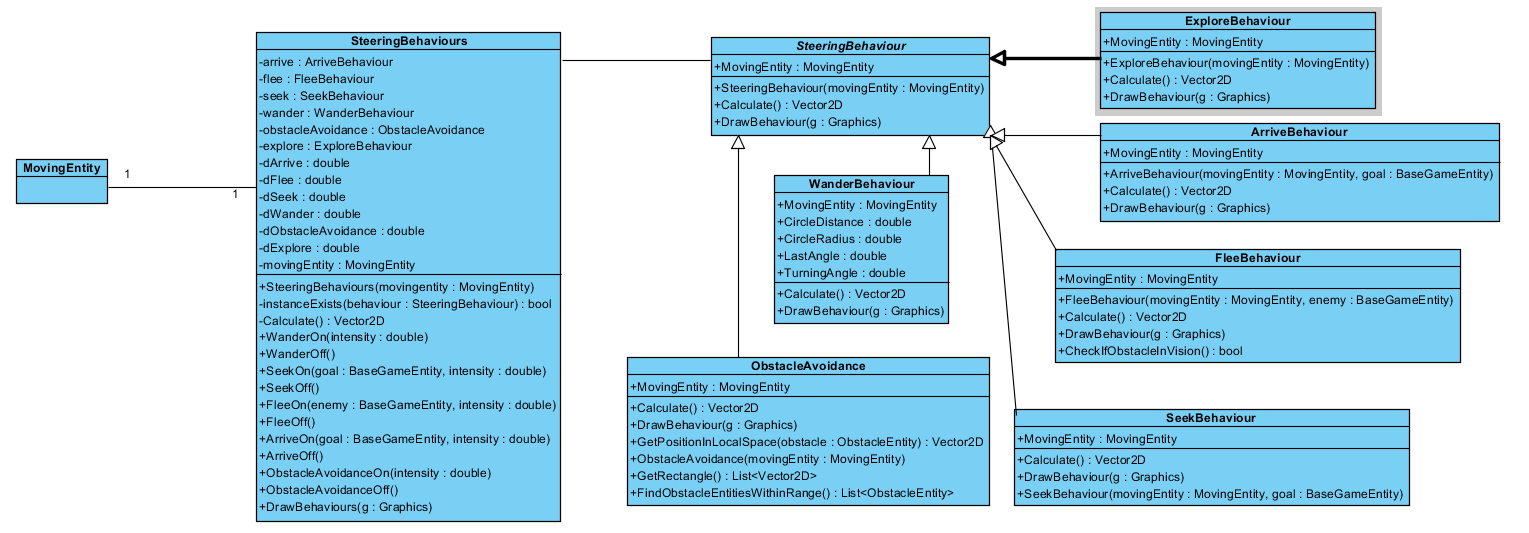
\includegraphics[width=35em]{BehavioursClassDiagram.PNG}
    \end{center}
    \caption{Steering behaviours class diagram}
    \label{fig:SteeringBehavioursClassDiagram}
\end{figure}
\newpage
%-----------------------------------------------------------------------------------------